% !TEX root = ../Main.tex

\chapter{Introduction}\label{chap:introduction}
% Quantum computers are emerging technology
% Widely expected to offer exponential advatnage over classical devices
% By definition, should not be clasically simulable
% Notion of this gap not yet understood
% Classical simulation probes this boundary
Over the past 10 years, quantum computation has rapidly transitioned from a field of research into a burgeoning industry, drawing attention from national governments~\cite{UKNQTP,QuantumFlagship}, and private enterprise~\cite{IBMQ,GoogleQuantum,MicrosoftQuantum} alike. This intense interest is driven by the expectation that quantum computers can perform exponentially faster than current, classical devices on certain computational tasks.\par
The kinds of problems that are expected to have such a `quantum advantage' are not only limited to simulating quantum mechanical systems~\cite{Lloyd1996}, including applications to chemistry and materials science~\cite{Brown2010}, but also include a tasks as diverse as optimization~\cite{Moll2018}, search~\cite{Grover1996}, prime factorization~\cite{Shor1994}, random walk algorithms~\cite{Kendon2006}, and linear algebra~\cite{Harrow2009}, including applications to machine learning~\cite{Biamonte2017}.\par
A natural consequence of this exponential separation in computational power is that any classical simulation of a quantum computer should in general require exponentially more time to complete. This might seem to preclude classical simulations as a means of studying the development of quantum computing.\par
However, in practice, classical simulations have proven to be a valuable tool in aiding the development of quantum computing. Firstly, as a practical tool; despite their expense, classical simulations of small systems can be used to study the performance of possible quantum hardware~\cite{Cai2019}. They also provide theorists and developers with explicit ways to verify quantum algorithms on limited numbers of qubits, and have the potential to support the newly emerging group of quantum software developers~\cite{Qiskit,MicrosoftQDK,CircAnnouncement}.\par
But classical simulations can also play an interesting role in the foundations of quantum information science. For example, by studying classical descriptions of quantum computing states and operations, we can identify cases with efficient classical representations. By definition, these restricted models of quantum computing cannot outperform a classical device, and thus probing the boundaries of these restricted models gives us a way to study the transition between classical and quantum computing.\par
This thesis presents a powerful method for classical simulations of quantum circuits, based on decompositions into circuits and states belonging to an efficiently simulable restricted model of quantum computation. The remaining chapters will outline the core components of this method. Here, we discuss the principles of quantum computing and some of the current understanding of the separation between quantum and classical paradigms. We then introduce different classical descriptions of quantum computing, and conclude by discussing different aspects of classical simulations based on these descriptions.
\section{Foundations of Quantum Computing}
% Feynmann, physics of computation link, MIT conference and physical turing machines
The development of quantum computing is has its origins in discussions on the connection between computation and physics. In particular, how can a computation be understood in terms of a physical system? Formally, we are interested in constructing a representation relation, such that inputs to the computational task can be encoded as physical parameters, and that a measurable property of the system can be decoded as a computational output~\cite{Horsman2014}. An interesting example of this kind of physical computation is the MONIAC, a macroeconomic simulator realised using fluid dynamics~\cite{Bissell2007}.\par
Given this kind of correspondence, we can then ask what insights physics can give into computation, and vice-versa. For example, it can be shown that analogue computation has the potential to efficiently solve $\NP$-hard problems~\cite{Schonhage1979}, for which it is widely believed no efficient discrete algorithm exists ($\P \neq \NP$, c.f.\ Section~\ref{sec:complexity}). The caveat, however, is that such a device would require arbitrarily high precision, and subsequently according to the Berkenstein bound would need infinite energy to operate~\cite{Aaronson2005}.\par
Alternatively, we can consider spin-glasses, a class of many-body Hamiltonian. It can be shown that computing the ground-state of a spin glass is $\NP$-hard~\cite{Barahona1982}, and it is possible to construct spin-glass Hamiltonians such that their ground-state corresponds to the solution to optimization problems~\cite{Choi2010,Lucas2014}. However, spin-glasses are also metastable, with the property that they `freeze' into higher energy configurations, and rendering it difficult to bring the system to its ground state~\cite{Edwards1975}. Adiabatic methods, where the spin-glass Hamiltonian is slowly turned on such that the system should stay in its ground-state configuration, can be shown to require exponentially long anneal times. From these two examples, there thus seems to be an equivalence between the difficulty of the computational task, and the physical realisation.\par
The first proposals for a quantum computer are widely attributed to the first conference on Physics of Computation, held at MIT in 1982. At that conference, Paul Benioff presented a way of realising a Turing machine using a quantum mechanical system of spins~\cite{Benioff1980}.\par
A Turing machine is an abstract model of computation, introduced to aid the study for classical computation~\cite{Nielsen2000}. In this model, the computer is made up of a `tape', discrete cells capable of storing a single value each, and a `head', capable of reading or writing a value to the tape, or moving left and right. At each time-step, the head performs one movement, read, write operation, or else terminates the programme. Importantly, the Church-Turing thesis states that \emph{any} computable function can be computed in finite time by a Turing machine. A Turing machine is a `universal' model of computation, and any system capable of realising a Turing machine is said to be `Turing Complete'~\cite{Nielsen2000}.\par
In this model, each spin encodes a single cell of the tape, and the programme would be realised by spin-spin interactions. However, while Benioff's proposal used quantum dynamics, and he argued that its direct realization on a physical system should make it highly efficient~\cite{Benioff1980}, the computational model was strictly classical.\par
In his keynote remarks at the same conference, Richard Feynman discussed the possibility of simulating quantum mechanical systems with classical computers. He argued that any classical simulation should require resources that scale exponentially in the size of the system, and also discussed a variant of the sign problem, arguing that this made classical simulation intractable~\cite{Feynman1982}. Instead, he discussed the option of building computers distinct from the Turing maching, out of purely quantum mechanical pieces, such that they could be used to realise Hamiltonians homomporphic to the process we want to simulate. These quantum computers, he proposed, could also be built out of lattices of spin-$\frac{1}{2}$ systems, and as quantum mechanical objects they should in some sense be able to efficiently encode quantum physical systems~\cite{Feynman1982}.\par
The idea of a quantum computation device built using two-level quantum systems was formalised by Deutsch, who introduced a more general model of quantum computing called a Quantum Turing Machine (QTM)~\cite{Deutsch1985}. In a QTM, the cells of the tape and the processor head are now built up of two-level quantum mechanical systems, which were later dubbed qubits in subsequent work by Schumacher on quantum versions of classical information theory~\cite{Schumacher1995}. At each timestep, the head and tape apply one of a finite set of unitary operations, which are capable of generating a group dense in the group of all possible unitary operations on the Hilbert-space of $2^{n}$ dimensional quantum systems~\cite{Deutsch1985}.\par
Deutsch also proves several powerful features of the QTM model. Firstly, noting the correspondence between reversible classical dynamics, reversible computation~\cite{Toffoli1980}, and unitary evolution, he points out that the QTM is itself Turing complete, and thus universal for classical computing~\cite{Deutsch1985}. He also proves that the QTM is capable of simulating finite dimensional quantum systems, and thus includes the notion of a quantum simulator discussed by Feynman~\cite{Deutsch1985}.\par
Having defined this notion of a universal quantum computer, Deutsch also introduces an extension of the Church-Turing thesis that relates computation more closely to physical systems. Today known as the Church-Turing-Deutsch thesis, it states
\begin{quote}
Every finitely realizable physical system can be perfectly simulated by a universal model computing machine operating by finite means.
\end{quote}
The QTM, as defined, satisfies this thesis, as it is capable of simulating finite quantum mechanical systems. However, the Turing machine fails this criteria for both classical and quantum physics, as continuously valued systems cannot be efficiently encoded in binary arithmetic~\cite{Deutsch1985}.
\subsection{Complexity Theory and Quantum Advantage}\label{sec:complexity}
%Basic notions of complexity theory: P, NP, PH, BQP
The Church-Turing-Deutsch thesis, inspired by Feynman's intuition, thus gives the first example of a gap in the computational power of quantum and classical devices. In this section, we will discuss this potential separation using computational complexity theory, and define more precisely the notion of a task being computationally `hard'.\par
Computational complexity theory is the study of computation by quantifying how the required number of operations, called `temporal complexity', and the amount of memory, called `spatial complexity', for computing given task scales as asymptotically as a function of the input parameters; typically, the `size' of the problem input~\cite{Nielsen2000}. As an abstract model of computing, we can relate the temporal and spatial complexity to the Turing machine; in this case, the number of steps taken by the head, and the number of cells on the tape.\par
However, typically, computational complexity doesn't deal with the Turing machine directly, instead reasoning based on models like boolean circuits, such that any computation in this model can be mapped to a Turing machine with at most a polynomial increase in the spatial or temporal complexity. A similar mapping exists for the QTM, which is the quantum circuit model widely used in quantum computing~\cite{Yao1993}.\par
\subsubsection*{Common Complexity Classes}
Complexity theory is generally interested in grouping problems into `classes', based on their asymptotic complexity, and studying the relationships between different classes. Provable membership of a class sets upper and lower-bounds on the performance of algorithms~\cite{Nielsen2000}.\par
Typically, in complexity theory, a task is considered `efficient' if its runtime is polynomial in the input size $n$. Given a deterministic algorithm to solve a problem efficiently, that problem belongs to the corresponding complexity class $\P$. Otherwise, algorithms with super-polynomial  scaling are considered `inefficient'. While this separation seems coarse, as an algorithm with scaling $O\left(a^{0.1n}\right)$ would scale more efficiently than a method that scales as $O(n^{1000})$, in practice problems in $\P$ perform better than those with exponential scaling~\cite{Nielsen2000}.\par
Algorithms can also be probabilistic; in the Turing machine model, this corresponds to allowing the program to pick a move at random based on some probability distribution. $\PP$, for `Probabilistic Polynomial', is the class of problems for which a probabilistic algorithm exists that fails with probability $p_{f}<\frac{1}{2}$. By running this algorithm repeatedly, such that the failure probability $p^{m}$ becomes arbitrarily small, but this can in practice require a large number of repetitions if for example $p=\frac{1}{2}-\frac{1}{2^{n}}$~\cite{Aaronson2004c}. Thus, the related class $\BPP$, Bounded Probabilistic Polynomial, is defined as problems where the failure probability $p < \frac{1}{3}$, such that the failure probability is exponentially decreasing in the number of repetitions~\cite{Nielsen2000}. It is immediately apparent that $\P\subseteq \BPP$, by setting $p_{f}=0$, and that $\BPP\subseteq \PP$.\par
Another common class considered is $\NP$, that class of problems for which a candidate solution can be checked in polynomial time, using a piece of additional information called a `witness' or `proof'. A common example is finding the factors of a number, which can be checked by multiplying the factors together. Importantly, however, there is not necessarily an efficient polynomial algorithm to find the solutions.\par
The class takes its name from the set of problems that can be efficiently solved by a `non-deterministic' Turing machine, which can be conceptualised as similar to a probabilistic Turing machine, but where the machine chooses the `best' path at each branching point such that it arrives at a solution.\par
$\P\subseteq \NP$, as any solution for a $\P$ problem can be efficiently checked by running the algorithm and comparing the solutions. Interestingly, if we allow for post-selection in a probabilistic computation, then we can see from our heuristic description of the nondeterministic Turing machine that $\NP\subseteq \PostBPP$. It can also be shown that $\NP\subseteq \PP$~\cite{Gill1974}.\par
The class $\NP$ contains many `interesting' problems for which an efficient classical algorithm is not known to exist~\cite{Nielsen2000}. In fact, many of these problems, including optimization tasks like the Traveling Salesman Problem, are called $\NP$-complete. A problem $P$ is said to be `complete' for a given complexity class if it is a member of that class, and if it satisfies an additional criterion called `hardness'. $P$ is said to be $\mathbf{C}$-hard if there exists an efficient `reduction' or mapping from all problems in $\mathbf{C}$ to $P$. Given an efficient algorithm to solve $P$, this then implies we can use the reduction to efficiently solve all problems in $\mathbf{C}$~\cite{Nielsen2000}.\par
Finally, we can also define spatial equivalents of complexity classes. $\P\SPACE$ is the class of all problems that can be solved requiring at most a polynomial amount of memory. Intuitively, this can also be thought of as the class of all problems that can be efficiently specified. We can also define exponential versions of the temporal and spatial complexity classes, $\EXP$ and $\EXPSPACE$, which leads to the following inclusion relation:
\[\P\subseteq\BPP\subseteq \NP \subseteq \P\SPACE \subseteq \EXP \subseteq \EXPSPACE. \]
Finally, here we briefly introduce two open questions in computational complexity that are nonetheless widely assumed to be false~\cite{Nielsen2000}.
\begin{align}
    \P &\neq\NP.\\
    \text{The Polynomial Hierarchy } &\PH \text{ does not collapse.}
\end{align}
Both of these results are typically invoked in `no-go' arguments when reasoning about computational complexity. $\P\neq \NP$ can also be stated as asserting that no polynomial time algorithm exists for $\NP$-complete problems. Scott Aaronson has discussed a number of arguments, from the physical to the philosophical, as to why we expect this to be the case~\cite{Aaronson2005,Aaronson2006}. Intuitively, $\P=\NP$ can be expressed as implying there's `no fundamental gap between finding a solution, and recognising a solution once it is found'~\cite{Aaronson2006}.\par
The Polynomial hierarchy is a recursively defined, infinite hierarchy of complexity classes that generalise $\P$ and $\NP$. A collapse of the Polynomial hierarchy would imply that the hierarchy is finite. This statement is closely related to class $\#\P$, which captures the complexity of problems where we are asked to count the number of valid solutions. Requiring the Polynomial Hierarchy to be infinite can be understood as expecting $\#\P$ problems to still be hard even if we are able to approximately count solutions~\cite{Dalzell2017}.
\subsubsection*{Quantum Computational Complexity}
% Quantum Complexity Classes
We can also define analogues of these complexity classes for quantum computation, using the QTM.\ The class considered `efficient' for quantum algorithms is $\BQP$, Bounded Quantum Polynomial; problems for which a polynomial time quantum algorithm exists with a bounded failure probability $p_{f}<\frac{1}{3}$~\cite{Nielsen2000}. Following Deutsch's observation that a QTM is capable of reversible classical computation, it can be shown that $\P\subseteq \BQP$~\cite{Bernstein1997}. The same paper also proved that a quantum computation on $T$ steps requires just $O\left(\log{T}\right)$ precision. Thus, if $\P\neq \BQP$, this super-classical advantage doesn't require arbitrary precision, as in the analogue computing case~\cite{Bernstein1997}.\par
The quantum class considered analogous to $\NP$ is $\QMA$, where there exists a polynomial time quantum algorithm that can verify a (quantum) solution with failure probability $p_{f}<\frac{1}{3}$~\cite{Watrous2008}. Examples of problems complete for $\QMA$ include deciding if a Hamiltonian built of just local interactions has a spectral gap~\cite{Kempe2004}.\par
Related to classical classes, it can be shown that $\BQP\subseteq \QMA\subseteq \PP$. However, it is believed that $\QMA\neq \PP$, as otherwise $\PH\subseteq \PP$~\cite{Vyalyi03}. The addition of post-selection however, as in the classical case, significantly boosts the capabilities of a quantum computer, and it can be shown that even $\PostBQP=\PP$~\cite{Aaronson2004c}.\par
$\QMA$ is also closely related to the class $\MA$, where we instead have a classical algorithm that can verify a solution with high probability given a classical proof. We can also define a `half-way' class between the two, where we allow for a quantum algorithm with just classical proof, and it can be shown that $\MA\subseteq \QCMA\subseteq \QMA$~\cite{Aharonov2002}.\par
In 1994, Shor famously demonstrated an efficient quantum algorithm for prime factorization~\cite{Shor1994}. Prime factoring is demonstrably in $\NP$, as we can efficiently check by multiplying factors. No efficient classical method is known to exist for prime factorization, but it has also not been definitively proven that factorization $\notin \P$~\cite{Nielsen2000}. Shor's algorithm strongly suggests $\P\neq \BQP$, but this separation has not been definitively shown.\par
There is, however, evidence that $\NP\nsubseteq \BQP$. In particular, if we consider a quantum algorithm with access to an oracle for verifying $\NP$ problems, then it can be shown the runtime of this algorithm must be $O\left(2^{\frac{n}{2}}\right)$, a quadratic reduction compared to many classical methods for $\NP$ problems which scale as $O\left(2^{n}\right)$~\cite{Bennett1997}. Such an oracle can be efficiently implemented using a quantum circuit, equivalent to a reversible classical circuit for the verifier. It was shown by Grover that this bound on the complexity is tight, using a quantum algorithm now commonly referred to as Grover search~\cite{Grover1996}. Overall, these results give some insight into the boundaries of $\BQP$. These are represented schematically in Figure~\ref{fig:bqp_venn}.
\begin{figure}
\centering
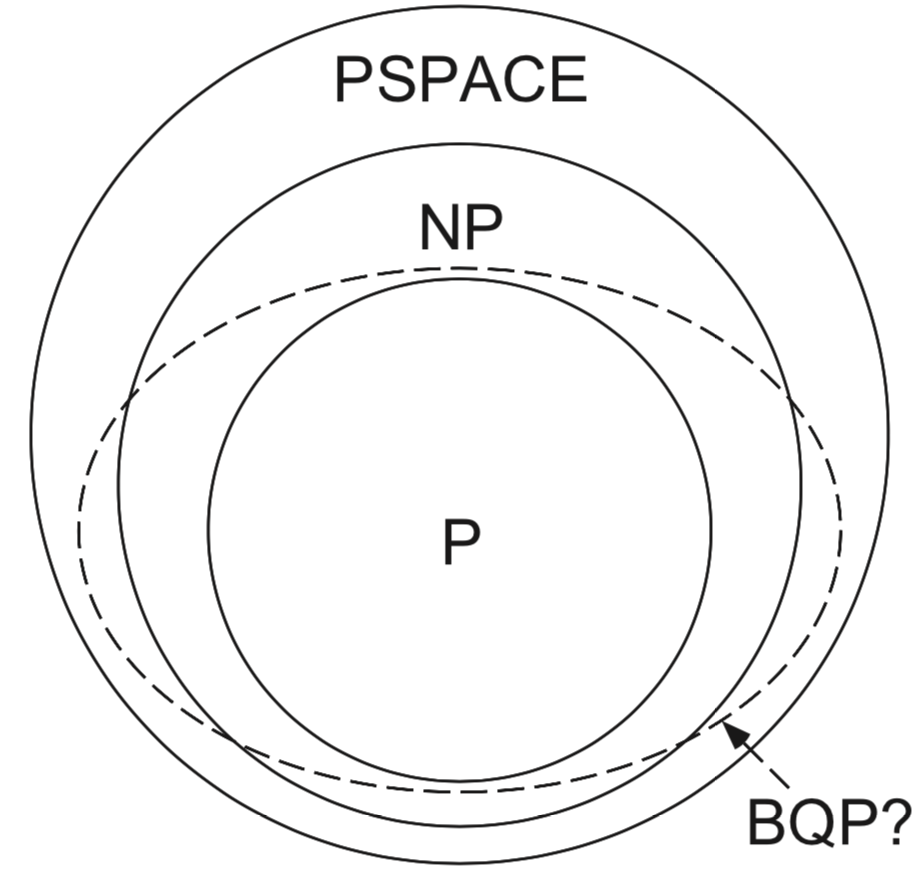
\includegraphics[width=0.75\textwidth]{Figures/BQP_diagram.png}
\caption{A Venn-diagram, illustrating the relationship of $\BQP$ to other classical complexity classes. Figure taken from~\cite{Nielsen2000}.}\label{fig:bqp_venn}
\end{figure}
%Spatial results???
\section{Classical Simulations of Quantum Computation}\label{sec:intro_classical_simulation}
The previous section discussed formal notions of quantum computation, and examined its relation to classical computation through the lens of complexity theory. In this section we will introduce classical descriptions of quantum computation. These can be thought of as a reduction from quantum computing to classical computation. Our classical discription, and simulation, are efficient then we can as a result efficiently simulate a quantum computation. We will begin introducing more precise notions of classical simulation, before focusing on different classical descriptions of quantum systems. This is by no means an exhaustive survey, but introduces some common paradigms for classical simulation. Finally, we will discuss results on the hardness of classical simulation, and briefly introduce the notion of a `quantum supremacy' test.
\subsection{Definitions of Classical Simulations}\label{sec:intro_simulation_types}
% Types of approximation
% Strong sampling
%  Weak sampling
The general structure of quantum computations involves preparing an initial quantum state $\ket{0^{\otimes n}}$, applying a unitary evolution $U$, and then applying a measurement or otherwise estimating an observable. Given this, an most obvious definition of classical simulation is to compute the probabilities of different observables on the final state $\ket{\psi}=U\ket{0^{\otimes n}}$. This task is typically called `strong' classical simulation~\cite{VandenNest2008}.
\begin{defn}[Strong Classical Simulation]\label{def:strong_simulation}
a strong classical simulator is any classical algorithm $\mathcal{A}$ that takes as input a description of a circuit $U$, and a description of the output observable $s$, and returns the probability of that output $p_{U}\left(s\right)$~\cite{VandenNest2008}.
\end{defn}
Here, $s$ could be the probability of some $n$-qubit computational state, or a marginal probability obtained by measuring some subset of the qubits. We denote as $\mathbf{S}$ the set of observables we are interested in simulating, and $\mathcal{P}_{\mathbf{S}}$ is the distribution of those events.\par
However, this task is distinct from what we are typically asking a quantum computer to do. When running a quantum algorithm, we are instead preparing the final state $\ket{\psi}$, and then sampling from its output distribution. These samples are then post-processed to estimate other observables.
\begin{defn}[Weak Classical Simulation]\label{def:weak_simulation}
A weak classical simulator is a classical algorithm $\mathcal{A}$ capable of taking a classical description of a circuit $U$, and returning samples from its output distribution $\mathcal{P}_{\mathbf{S}}$~\cite{VandenNest2008}.
\end{defn}
A weak simulator can be conceptualised as equivalent to having access to a quantum computer itself~\cite{Pashayan2017}.\par
In practice quantum computations are not perfectly accurate, due to the influence of physical noise and control errors. We can correspondingly relax our definitions of classical simulation, to allow for a degree of approximation. An approximate strong simulation computes a given probability to within some specified precision $\epsilon$, and an approximate weak simulation allows us to sample from a distribution $\mathcal{\hat{P}}_{\mathbf{S}}$ that approximates $\mathcal{P}_{\mathbf{S}}$.\par
There are several different definitions of precision used in approximate classical simulation. For strong simulation, there are three common definitions:
\begin{defn}[Approximate Strong Simulation]\label{def:approximate_strong}
An approximate strong simulator computes estimates of output probabilities $\hat{p}\left(s\right)$ to within a given error $\epsilon$, that is either
\begin{enumerate}
    \item \textbf{Additive}: $\left|p\left(s\right)-\hat{p}\left(s\right)\right| \leq \epsilon\;\forall s\in\mathbf{S}$~\cite{Pashayan2017}
    \item \textbf{Multiplicative}: $\frac{1}{\epsilon}p\left(s\right)\leq \hat{p}\left(s\right) \leq \epsilon p\left(s\right)\;\forall s\in\mathbf{S}$~\cite{Hangleiter2017}
    \item \textbf{Relative}: $\left(1-\epsilon\right)p\left(s\right) \leq \hat{p}\left(s\right) \leq \left(1+\epsilon\right)p\left(s\right) \;\forall s\in\mathbf{S} $~\cite{Bravyi2016,Hangleiter2017}.
\end{enumerate}
\end{defn}
Multiplicative and relative precision are slightly stronger requirements than additive error, as can be seen by considering the case where $p\left(s\right)\rightarrow 0$. In the literature, `relative' simulation is also sometimes referred to as `multiplicative' simulation, as the condition can be rewritten as~\cite{Pashayan2017}
\[\left|p\left(s\right)-\hat{p}\left(s\right)\right| \leq \epsilon p\left(s\right).\]
For weak simulation, there is one commonly used notion of precision that is variously referred to as $\ell_{1}$-precision~\cite{Bremner2011}, additive precision~\cite{Yoganathan2019} or simply $\epsilon$-precision~\cite{Pashayan2017}.
\begin{defn}[Approximate Weak Simulation]\label{def:approximate_weak}
An approximate weak simulator samples from an output distribution $\hat{\mathcal{P}}$ such that
\[ \norm{\mathcal{P}_{\mathbf{S}}-\hat{\mathcal{P}}_{\mathbf{S}}}_{1} = \sum_{s\in \mathbf{S}} \left| p\left(s\right) - \hat{p}\left(s\right)\right| \leq \epsilon.\]
\end{defn}
The use of the one-norm is motivated as the one-norm is directly proportional to the total variational distance between the two distributions.\par
Sometimes, a classical algorithm is capable of generating an approximate simulation $\hat{q}$ with some precision $f\left(\epsilon\right)$, with a non-zero probability of failure such that
\[\text{Pr}\left[\left|q-\hat{q}\right| > f\left(\epsilon\right)\right]\leq \delta.\]
This is referred to as an $\left(\epsilon,\,\delta\right)$-precision approximation~\cite{Pashayan2017}. If this precision $\delta$ is bounded, then by $m$ repeat rounds the probability of failure can be reduced to $\delta^{m}$, as in the case for the complexity class $\BPP$.\par
Given these notions then, we can define an efficient $\left(\epsilon,\,\delta\right)$-approximate classical simulation of an $n$ qubit system as one with a complexity that scales as $\poly \left(n, \epsilon^{-1}, \log{\delta^{-1}}\right)$~\cite{Pashayan2017}.
\subsection{Classical Descriptions of Quantum Systems}\label{sec:intro_classical_desc}
% statevector methods & p-blockedness
What could be called the `textbook' description of a quantum computation is the state-vector representation, a vector $\ket{\psi}\in\mathbb{C}^{2^{n}}$ that encodes the wave-function of the $n$-qubit system~\cite{Nielsen2000}. In this picture, the state is updated by applying $2^{n}\times 2^{n}$ unitary matrices. Thus, simulating a quantum computation in this picture might seem to require exponential spatial and temporal resources.\par
However, as quantum circuits are typically built out of local interactions, usually $1$ and $2$ qubit gates, it is possible build block decompositions of both the state-vector and unitary matrices. While a general state-vector requires $2^{n}$ complex numbers to completely specify, a tensor-product of smaller states requires just $O\left(n\right)$~\cite{Ekert1998}.\par
A quantum computation can be described as $p$-blocked if at all time-points it can be decomposed into a tensor product of subsystems each acting on at most $p$ qubits, where $1\leq p\leq n$~\cite{Jozsa2003}. It can be shown that the complexity of both strong and weak classical simulation on a $p$-blocked state-vector has a running time that scales as $O(2^{p+1}\poly\left(m\right))$, where $m$ is the number of blocks~\cite{Jozsa2003}. If $p$ grows at most logarithmically in the system size, then this simulation is efficient, and for a fixed $p$ further increases in system size are efficient. Otherwise, if $p$ grows unboundedly with the duration of the computation, then simulation requires exponential resources. Interestingly, it can be shown that for example in Shor's algorithm, $p=n$~\cite{Ekert1998}.\par
% Other methods like the binary search trees JMK thingy
The Quantum Multiple Decision Diagram (QMDD) is an alternative encoding of the state-vector that similarly exploits redundancies arising from terms with equal amplitudes~\cite{Niemann2016}. They combine this with a tree-based data-structure, where each leaf of the tree corresponds to a distinct amplitude, labelled by the outcomes to which it corresponds. In general, an arbitrary QMDD will have $2^{n}$ leaves, but the authors show that in practice QMDDs can be significantly smaller than this during common routines including the Quantum Fourier Transform, and this can be exploited to develop a classical simulation method where updates scale as $O\left(n \left|v\right|\right)$, where $\left|v\right|$ is the number of leaves in the tree~\cite{Zulehner2017}. If this number grows at most polynomially in the system size, the simulation is efficient.\par
% Approximate QMDD => sparseness, as in VdN
The cases where $\left|v\right|$ grows at most polynomially in the system size corresponds to the definiton of computationally tractable states, classes of states that admit efficient strong and weak simulation in the computational basis~\cite{VandenNest2009}. Certain sparse circuits acting on computationally tractable state in turn produce a computationally tractable output state, and thus can be efficiently simulated. This definition can also be expanded to approximate simulation, where we approximate its output distribution $\mathcal{P}$ to within additive error $\epsilon$, with some other distribution $\mathcal{\hat{P}}$ that is computationally tractable~\cite{Schwarz2013}.\par
% Tensor network descriptions, alternative picture
An alternative representation of a quantum circuit, that is more disticnt from the state-vector picture, is the use of tensor networks to simulate quantum circuits. These methods were first introduced in the context of simulating dynamics of many-body quantum systems~\cite{Vidal2003}.\par
Tensor networks are undirected graphs, where tensors represent input and output states, and quantum gates, and edges represent qubit wires~\cite{Markov2005}. Tensors are combined or contracted by summing over shared indices, with a runtime that scales as the product of the dimensions of the indices to be contracted. For fixed input and output states $x$ and $y$, contracting the entire network results in a rank-0 tensor or scalar value which corresponds to the amplitude $\matrixel{x}{u}{y}$~\cite{Markov2005}. It can be shown that the complexity of simulating a tensor network scales exponentially with the `tree-width', a property of the underlying graph of the network~\cite{Markov2005}. In general, tensor networks are known to be efficient when the entanglement of the system is bounded~\cite{Vidal2003}. It can also be shown that for circuits built out of one and two-qubit gates, the tree-width scales linearly with both the number of qubits and the cirucit depth~\cite{Markov2005}.\par
% Wigner function picture, born from QO and gaussian states
An alternative classical description of quantum circuits commonly discussed in the literature are quasiprobability or `Wigner function' representations~\cite{Wootters1987}. In this picture, the state is encoded in a quasiprobability distribution on a phase-space, where each point is described by a set of mutually anti-commuting operators~\cite{Wootters1987}. The phase-space can be continuous, as is used in the study of quantum optics~\cite{Nielsen2000}, or discrete, as is usually considered in the context of quantum computing~\cite{Gross2006}.\par
It can be shown that, if the Wigner function representation is strictly positive, then the system is efficiently simulable classically~\cite{Bartlett2002,Mari2012}. This is analogous to the same sign-problem discussed by Feynman in his 1982 address~\cite{Feynman1982}. Positive Wigner function simulations use a random walk across the phase-space, with transition probabilities given by Wigner function expansions of each gate $U$. If the Wigner function is negative, then it is possible to define an alternative sampling strategy that can be used to simulate the computation, but at the expense of an increase in the number of samples, which scales exponentially `negativity' of the system, the one-norm of its quasiprobability expansion~\cite{Pashayan2015}. The negativity is by definition $1$ if the system is non-negative, and $>1$ otherwise.
\subsection{Efficiently Simulable Quantum Systems}\label{sec:intro_efficient_simulations}
% Prop D note from Jozsa et al
In the previous section, we introduced several different representations of quantum computations used in classical simulations. In each case, there are also certain circumstances under which the simulation is efficient. Indeed, in their paper on simulation of $p$-blocked computations, it was noted by Jozsa \& Linden that in general for any classical description $\mathcal{D}$, then there exists a corresponding property $\text{prop}\left(\mathcal{D}\right)$ that is required for the simulation to be intractable classically~\cite{Jozsa2003}. For example, in both the $p$-blocked picture and the tensor network picture, the required feature $\text{prop}\left(\mathcal{D}\right)$ is that the entanglement in the system grow unboundedly during the computation~\cite{Jozsa2003,Vidal2003}.\par
% E.g. stabilizer states, explore in detail
Perhaps the most famous example of this requirement is related to the Gottesman-Knill theorem~\cite{Gottesman1998b,Jozsa2003}.
\begin{quote}
\textbf{Gottesman-Knill Theorem:} A quantum circuit built out of only 
\begin{itemize}
    \item Preparation of states in the computational basis
    \item Clifford and Pauli gates
    \item Measurement in the computational basis
\end{itemize}
can be efficiently simulated on a classical computer.
\end{quote}
We will discuss the Gottesman-Knill theorem and how these circuits, typically called stabilizer circuits, can be simulated in Chapter~\ref{chap:stabilizers}. This theorem has gained particular attention in the field for several reasons. Firstly, it sets up a clear correspondence between classical simulability and universal quantum computing. The gate-set of stabilizer circuits is not universal for quantum computation. This means these circuits cannot be used to build up arbitrary unitary operations~\cite{Nielsen2000}. In fact, stabilizer circuits are also not universal for classical computation~\cite{Aaronson2004}. However, introducing a single gate outside of this set is sufficient to generate a group dense in the special unitary group, and thus `promote' the gate-set to universality.\par
Stabilizer circuits are also closely related to the study of quantum error-correcting codes, where logical gates `native' to he code are typically Pauli and Clifford gates corresponding to stabilizer circuits~\cite{Nielsen2000}. Non-Clifford gates are then introduced through a protocol called state-injection, involving `magic' states that cannot be generated by stabilizer circuits~\cite{Gottesman1999,Bravyi2005}.\par
Interestingly, it has also been shown that there is a correspondence between stabilizer circuits, and `contextuality', a generalised notion of locality~\cite{Howard2014}. Contextuality was first discussed in the 1960s, where it was argued that non-contextuality is a unique feature of quantum systems~\cite{Bell1966,Kochen1967}. For example, in Spekkens's Toy Model, a classical model of quantum systems based on a restriction of available information, features like non-locality and entanglement can be efficiently described, but non-contextuality cannot~\cite{Kochen1967}. Similarly, it was shown by Howard et al.\ that in odd-prime dimensional quantum systems, stabilizer circuits are entirely contextual, and the onset of non-contextuality is connected to the ability to distill high-fidelity magics states~\cite{Howard2014}. The case is slightly more complicated for quantum computing with qubits, as qubits show state-independent contextuality, but recent work has extended this correspondence between contextuality and qubit magic states~\cite{BermejoVega2017}.
\subsubsection*{Resources for Quantum Computation}
% Prod D and resources
The Gottesman-Knill theorem makes it clear that non-stabilizer resources are required for universal quantum computation, and as stated there is a correspondence between this required property and classical simulability. In fact, in general, the property $\text{prop}\left(\mathcal{D}\right)$ can be interpreted as `required' for quantum advantage, from the corresponding breakdown of efficient classical simulation. Jozsa \& Linden argue that rather than any one `true' $\text{prop}\left(\mathcal{D}\right)$, it is likely that quantum computation requires all of these properties to be true.\par
% Examples
For example, as discussed in the $p$-blocked case, this suggests that entanglement is required for quantum advantage. However, given that entangled stabilizer circuits exist, entanglement alone is clearly not sufficient. Similarly however, it is easy to construct non-stabilizer circuits that are either $p$-blocked, or sparse such that the output is computationally tractable.\par
The study of these potential resources, not only for computation but also for non-classical phenomena more generally, are called quantum resource theories. In general, a quantum resource theory is composed of a set of states that are considered `free', a set of states that have an associated `cost', and a set of allowed or `free' operations~\cite{Brandao2015}. We are then interested in asking what is the associated resource cost of certain protocols, and how does the resource behave under free operations?\par
Resource theories have been applied to a broad range of phenomena, including; non-stabilizer states~\cite{Veitch2014}; magic states~\cite{Howard2017}, more specifically; and asymmetry~\cite{Piani2016}, which relates to both computational tractability~\cite{VandenNest2009} and to generalizations of Gottesman-Knill called normalizer circuits~\cite{BermejoVega2014}. Of particular interest a resource theories where the set of free states is convex, as these also admit convex cost functions that can be more easily analysed~\cite{Regula2018}. All of the examples given in this paragraph fall into the category of convex resource theories~\cite{Chitambar2019}.\par
% Simulation schemes w/ wigner function
There is also typically a correspondence between free states and operations in resource theories and their classical simulability. Indeed, many of the resource theories discussed above explicitly admit classical simulation through a discrete Wigner function representation. For example, it can be proven that any mixed state on $n$ qubits with a positive Wigner function representation can be described as a convex mixture of stabilizer states~\cite{Gross2006}. In these pictures, the resource cost of a given state is directly related to the computational cost of classical simulation~\cite{Howard2017,Kocia2017,Seddon2019,Raussendorf2019}.\par
As an example of the power of resource theories, we can consider the Robustness of Magic (RoM), introduced in~\cite{Howard2017}. This measure is equal to the negativity of a stabilizer state decomposition of a state. The RoM is largest for pure, non-stabilizer states, which lie outside the convex hull of the stabilizer states. However, as the state we are considering becomes more and more mixed, for example as a result of environment noise, it is pushed closer to the set of free states. Below some threshold, the state has RoM $\mathcal{R}\left(\rho\right)=1$, and can be efficiently simulated. This corresponds neatly with the notion of magic state distillation, where we are trying to `distill' pure magic states using Clifford circuits. We are consuming multiple copies, to produce a magic state with increased robustness, and which is subsequently harder to classically simulate. It is also congruous with the existence of a noise threshold below which we cannot distill~\cite{Bravyi2005}; below this threshold, the `noisy' magic states are `free' states, and thus we cannot increase their RoM using just free operations.
%TODO: Add figure???
\subsection{Simulation and Quantum Advantage}\label{sec:intro_complexity}
Given some of the results quoted in the previous sections, we might imagine that a sufficiently optimized classical simulation could exist to simulate quantum circuits. Here, we will review results from complexity theory which suggest that even an approximate efficient classical simulation of arbitrary quantum computation should not be possible.\par
\subsubsection*{Hardness of Strong Simulation}
% Hardness of strong simulation
% Encodes #P
It can be shown that exact strong simulation would imply the existence of efficient classical algorithms to solve problems in $\#\P$, using a correspondence based on quantum circuits. From a famous computational result in complexity theory called Toda's theorem, it can be shown that the complexity class of problems solvable by a $\P$ algorithm with access to an oracle for $\#\P$, typically denoted $\P^{\#\P}$, in fact contains the entire $\PH$~\cite{Toda1991}. Thus, the existence of an efficient classical algorithm for $\#\P$ problems would imply even strong consequences than $\P=\NP$.\par
The proof relies on the ability to construct quantum circuits $C$ out of $H$ and Toffoli gates~\cite{Dawson2004}, or alternatively out of $H$, $Z$, $CZ$ and $CCZ$ gates~\cite{Montanaro2017}, such that computing the probability amplitude 
\[\matrixel{0^{\otimes n}}{C}{0^{\otimes n}} \propto \text{gap}\left(f\right),\]
where $f\,:\,\{0,1\}^{n}\rightarrow \{0,1\}$ is an $n$-variable binary polynomial, and
\[\text{gap}\left(f\right) = \# \va{x}:f\left(\va{x}\right)=1 - \# \va{x}:f\left(\va{x}\right)=0.\]
This problem is known to be $\#\P$ hard in general, if $f$ has degree $\geq 3$~\cite{Montanaro2017}. Interestingly, this example also illustrates a case where studying quantum algorithms casts light on classical complexity theory. It was believed but not conclusively shown that $\text{gap}\left(f\right)$ could be efficiently computed for polynomials with degree $\leq 2$. A quantum circuit to compute the gap of such a polynomial could be built using just $H$, $Z$, and $CZ$ gates, and is thus a stabilizer circuit. This means the amplitude $\matrixel{0^{\otimes n}}{C}{0^{\otimes n}}$ can in turn be computed efficiently, resolving the open problem~\cite{Montanaro2017}. This example also further illuminates the relationship between stabilizer ciruits and classical computation; circuits built using $H$, $Z$, $CZ$ and $CCZ$ gates are known to be universal for quantum computing, and in turn are likely not to be strongly simulable.\par
% Hard to even approximate
% Relation to Ising Partition Funtions, matrix permanent
There is in fact evidence that approximate strong simulation of quantum computations would also imply the collapse of the $\PH$.
For example, there exists a $\BQP$ algorithm for approximately evaluating the Jones polynomial~\cite{Aharonov2007}, an important problem in the study of topological quantum field theories, to within additive error. This algorithm is based on repeatedly running a quantum circuit a polynomial number of times to obtain an estimate of a particular amplitude, and thus a strong classical simulation could be used to compute the Jones polynomial exactly. However, it can be shown that even approximating the Jones polynomial to within multiplicative error $\epsilon$ is a problem in $\#\P$~\cite{Kuperberg2009}, and thus no approximate strong classical simulation can exist unless the $\PH$ collapses. Interestingly, it is believed that approximately evaluating the Jones polynomial is a $\BQP$-complete problem, and thus this result would suggest that $\BQP$ problems cannot be efficiently strongly simulated classically.\par
A core lemma in the proof of~\cite{Kuperberg2009} is that given some family of quantum circuits $C$ such that, with the addition of post-selection, $\text{post}-C=\PostBQP$, then an efficient strong simulation of the output distribution of $C$ would collapse the polynomial hierarchy. For the Jones polynomial, this follows as the problem is $\BQP$-complete. Interestingly however, this result can also be used to imply that approximate strong simulation is hard even for certain types of quantum computation that are `weak' i.e.\ strictly not universal~\cite{Aaronson2010}. For example, Instantaneous Quantum Polynomial (IQP) circuits, circuits with depth $\poly\left(n\right)$, built out commuting gates like $Z$, $CZ$ and $CCZ$, have the property that they are universal under post-selection~\cite{Bremner2011}. Thus, strong simulation of IQP circuits implies the collapse of the $\PH$~\cite{Goldberg2014}.\par
An alternative strategy involves finding some correspondence between the quantum computation and another problem known to be $\#\P$ hard. For example, the output distribution of IQP circuits can be shown to be equivalent to partition functions of Ising model Hamiltonians~\cite{Fujii2017}, and thus from a characterisation of these partition functions IQP circuits are $\#\P$ hard to simulate in general~\cite{Goldberg2014}. This is also the strategy employed by Aaronson \& Arkhipov, when showing that a quantum optics task called Boson Sampling is equivalent to computing the permanent of a matrix to within additive error~\cite{Aaronson2010}, a known $\#\P$-hard problem~\cite{Valiant1979}.
% Acceptance probability?quant-ph/9812056
\subsubsection*{Extending Results to the Weak Simulation Case}
% Van den Nest, separation between strong and weak sampling
While the results above apply to strong classical simulation, as discussed weak simulation can be considered as a more appropriate definition of classical simulation. It was also shown by Van den Nest that it is possible to construct quantum circuits whose strong simulation can be proven to be in $\#\P$, but which nonetheless admit an efficient weak simulation~\cite{VandenNest2008}. Thus, a bound on strong simulation is not sufficient to rule out classical simulation of quantum circuits.\par
Initial evidence for the hardness of weak sampling was given in~\cite{Bremner2011}, who showed a weak simulation of IQP circuits with multiplicative error would imply the collapse of $\PH$. Here, multiplicative error means that we have some approximate distribution $\hat{\mathcal{P}}$, such that every term is itself a multiplicative approximate of the true probability. This is strong requirement for approximate classical simulation.\par
% Connecting approximate strong and weak computation
Subsequent work has shown that in fact, it is possible to lift a complexity theoretic bound on strong simulation with multiplicative error, to obtain an equivalent bound on weak simulation with additive error, given a proof that the circuit families satisfies a pair of conjectures called `anti-concentration' and `average-case hardness'~\cite{Hangleiter2017}. Recall that we are considering a family of quantum circuits $C$, which are hard to approximately strongly simulate, either as they are universal under postselection, or through correspondence to some other problem which is known to be $\#\P$-hard in the worst case.\par
The output distribution of these circuits is said to anticoncentrate if there exist two positive real numbers $\alpha$ and $\beta$, such that
\begin{equation}
\text{Pr}_{U\sim \mathcal{P}_{C}}\left(\left|\matrixel{x}{U}{0^{\otimes n}}\right|^{2}\geq \frac{\alpha}{N}\right) > \beta,
\label{eq:anticoncentration}
\end{equation}
where $N$ is the dimension of the system, typically $2^{n}$ for $n$ qubits~\cite{Hangleiter2017}. This theorem states that for some random circuit $U$ drawn from the family $C$, the probability of an arbitrarily chosen entry being greater than uniform is greater than $\beta$. Intuitively, anticoncentration requires that there is high probability the output distribution of $U$ is reasonably close to uniform~\cite{Harrow2017}. This ensures we are unlikely to find a circuit $U$ with an exactly or approximately sparse output distribution, that would be subsequently amenable to classical simulation~\cite{VandenNest2008,Schwarz2013}.\par
Average-case hardness requires that, given a problem that is known to be $\#\P$ hard to approximately compute in the worst-case, then it is also $\#\P$ hard to simulate on some constant fraction $c>0$ of the problem instance~\cite{Bremner2016}. This takes us from a family of problems that can in principle be hard to simulate, to one where there are many instances known to be hard to simulate~\cite{Harrow2017}. For example, some Ising Hamiltonians, and thus some instances of IQP circuits, are known to be classically simulable~\cite{Fujii2017}. Nonetheless, IQP circuits can be shown to satisfy average-case hardness~\cite{Bremner2016}.\par
These two properties can be combined with a result from classical complexity theory called the Stockmeyer Counting Algorithm~\cite{Stockmeyer1985}. Taken together, average-case hardness and anticoncentration imply that a classical simulator capable of sampling with a worst-case additive error is in fact capable of sampling with an average-case multiplicative error~\cite{Bremner2016}. Subsequently, using the Stockmeyer algorithm, this weak simulator can then be used to obtain an estimate of an output probability with multiplicative error. This completes the reduction from weak simulation with additive error, to strong simulation with multiplicative error, and thus shows that weak simulation is also $\#\P$-hard~\cite{Bremner2016}.\par
% Hakop paper about connecting estimating probabilties and sampling
% Polybox notion, strong additive approximation also insufficient for efficient sampling
Subsequent work has strengthened the case for the hardness of weak simulation. Consider having access to a classical algorithm capable of computing certain output probabilities with additive $\left(\epsilon,\delta\right)$-precision, efficiently --- namely, with a runtime that scales as $\poly\left(n,\epsilon^{-1},\log\delta^{-1}\right)$. Such a device is called a poly-box~\cite{Pashayan2017}. It can be shown that even with such a capability, the output distribution cannot be efficiently weakly simulated with additive error as long as the output distribution $\mathcal{P}$ is not approximately sparse. Namely, there does not exist some distribution $\hat{\mathcal{P}}$ such that $\norm{\mathcal{P}-\mathcal{\hat{P}}}\leq \epsilon$, and which has $t=\poly\left(\epsilon^{-1}\right)$ non-zero amplitudes. Namely, even with such a strong classical simulation device, the distribution cannot be weakly simulated if it is sufficiently dense.
\subsubsection*{Quantum `Supremacy'}
% Connection to quantum supremacy experiments
While not necessarily practically applicable, these kind of random problems that are believed to be hard to simulate clasically under the assumption the $\PH$ does not collapse form the basis of an effort in the quantum computing community to demonstrate so-called `quantum supremacy' --- the ability for a quantum computer to successfully run an algorithm super-polynomially faster than a classical computer~\cite{Preskill2012}.
\footnote{I want to acknowledge here the very real concerns that have been raised about the use of the word supremacy, given the historical and contemporary political significance of the word. I use the term in this thesis as, despite much discussion, it has become the \emph{de facto} name for this phenomenon.}
\par
These kind of random circuit problems are especially interesting compared to more direct tasks such as Shor's algorithm, because they require significantly fewer qubits to implement, and in some cases do not even require a universal architecture~\cite{Montanaro2017}. They are also more interesting than `analogue' quantum simulators, quantum systems that realise model Hamiltonians, as we have much strong guarantees on their computational hardness~\cite{Montanaro2017}. Nonetheless, there has been recent effort in the community towards constructing quantum simulators with provable hardness~\cite{Gao2017,BermejoVega2018,Hangleiter2017,Haferkamp2019}.\par
A quantum supremacy experiment based on these kind of random sampling problems with be made up of two key parts: sampling, and verification. The first task, also referred to as `Heavy Output Generation', is to generate a large number of samples from the output distribution of a given quantum circuit, drawn at random from a family of circuits~\cite{Aaronson2016}. This is done simultaneously using both a quantum computer, and an appropriate classical simulation method, presumably using High Performance Computing (HPC) resources.\par
The next step is to use an additional classical method to verify the output of both the quantum and classical samples. This step is in general even more computationally intensive than the sampling step, and is a significant caveat in current quantum supremacy proposals compared to running an $\NP$ problem such as factorization, which can be efficiently checked~\cite{Harrow2017}. After verification, the runtime and resources required for both the quantum and classical methods are compared.\par
An important caveat in realising quantum supremacy experiments, however, is their susceptibility to noise. As previously discussed, sufficiently noisy quantum computations can in fact be efficiently simulated classically. It is thus important that quantum supremacy protocols are reasonably robust, as quantum error correction is out of reach for contemporary quantum computers~\cite{Preskill2018}.\par
This caveat also acts in tandem with continued development of classical simulation methods. For example, recent effort in simulation of noisy boson sampling problems has pushed the threshold for quantum supremacy to around $30-40$ photons~\cite{Neville2017}, compared to current experimental records of about $6$.\par
Because noisy quantum circuits can typically be more easily simulated, an alternative proposal for quantum supremacy experiments changes the order of the classical sampling and verification steps. The idea is to use a classical verifier capable of estimating noise in the system~\cite{Villalonga2019}, such that this noise parameter can be used as input to the classical simulation to enable a fairer comparison.

